% Niveau :      PCSI
% Discipline :  Ondes
% Mots clés :   Breves

\begin{exercise}{Anharmonicité d'une corde de piano}{1}{Sup}
{Ondes,Corde}{lelay}

On s'intéresse aux modes propres d'une corde de piano de longueur $L$, fixée en ses deux extrémités. 

On peut montrer que la relation entre le vecteur d'onde et la pulsation d'une onde se propageant le long de cette corde est $\omega = ck \sqrt{1+ \alpha k^2}$, où $c$ et $\alpha$ dépendent de la section de la corde et de sa tension, mais pas de sa longueur.

Le coefficient $\alpha$ est dû à la raideur de la corde (il serait nul pour une corde parfaitement souple comme la corde de Melde).

\begin{questions}
    \questioncours Ondes le long d'une corde vibrante (corde de Melde), modes propres
    \question Quelles sont les valeurs possibles de $k$ pour une onde stationnaire existant sur cette corde ? Exprimer les fréquences correspondantes en fonction de $c$, $\alpha$, $L$ et d'un entier $n$.
    \question Les cordes d'un piano de concert sont plus longues que les cordes d'un piano de salon. Pourquoi cela améliore-t-il la qualité musicale du son ?
\end{questions}
\end{exercise}

\begin{exercise}{Réflexion d'une déformation}{2}{Sup}
{Ondes,Corde}{lelay}

On considère une corde de longueur $L$ qui s'étend de $x = 0$ à $x = L$. Un opérateur impose à l'extrémité le mouvement suivant :

$y(0, t) = 0$ pour $t \leq 0$
    
$y(0, t) = at/\tau$ pour $0 \leq t \leq \tau$
    
$y(0, t) = a(2\tau-t)$ pour $\tau \leq t \leq 2\tau$
    
puis laisse la corde au repos.

On considère $L = 10\ c\ \tau$, où $c$ est la célérité de propagation des ondes le long de la corde.
 
\begin{questions}
    \questioncours Propagation des ondes le long d'une corde
    \question Représenter l'allure de la corde à la date $t = 4\ \tau$
    \question On note $y_\text{i}(x, t) = F(x-ct)$ l'amplitude de l'onde incidente. Montrer qu'il existe nécessairement une onde réfléchie et déterminer son amplitude $y_\text{r}(x, t)$.
    \question En déduire la représentation de l'allure de la corde à $t = 11.5\  \tau$.
    \question On considère cette fois que l'extrémité de la corde, en $x=L$, peut coulisser sans frottements parallèlement à l'axe transverse $(Oy)$. Reprendre les deux questions précédentes avec cette nouvelle condition aux limites. On admet que la tension de la corde s'écrit $T(x, t) = T_0\pdv{y}{x}(x, t)$
\end{questions}
\end{exercise}


\begin{exercise}{Battements}{1}{Sup}
{Ondes,Battements}{lelay}

La figure ci-dessous présente l'enregistrement des battements de deux signaux sinusoïdaux produits par deux générateurs de basses fréquences. On demande de déterminer les fréquences des signaux ainsi que leurs amplitudes.
 
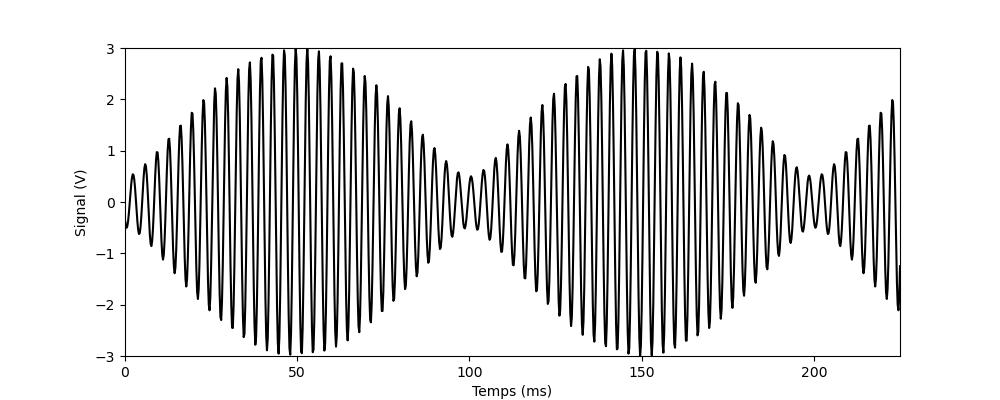
\includegraphics[width=0.95\textwidth]{propagation/battements.jpg}
\end{exercise}

\begin{solution}
Pour les fréquences, la porteuse a une demi-période de 100 ms et l'oscillation rapide fait 15 oscillations en 50 ms soit d'où $f_1 + f_2 = 600$~Hz et $f_1-f_2 = 10$~Hz et donc $f_1 = 295$~Hz et $f_2 = 305$~Hz.

Pour les amplitudes, $A_1 + A_2 = 3$ et $A_1- A_2 = 0.5$ d'où $A_1 = 1.25$ V et $A_2 = 1.75$ V
\end{solution}